\chapter{Temporal Topic Expertise Activity (TTEA)}
\doublespacing
\label{chap:ttea}
\minitoc




\section{Mining expertise and temporal information}

Chapter \ref{chap:qasm} proposed a method to formalize the latent information in user-generated content. The key point was how to extract these information. Chapter \ref{chap:lda} introduced the use of the original LDA model to extract topics and communities. In this chapter, we extend the results of chapter \ref{chap:lda} to extract topic based expertise and topic based temporal knowledge.

Let us consider StackOverflow for an example of the problem we address. In StackOverflow, For instance, \textit{Alice} posts a question at \textit{08/11/2015}, and assigns it with the tags \{\textit{html}, \textit{css}, \textit{height}\}. Her question then gets \textit{30} votes, and \textit{Bob} gives an answer to this question at \textit{10/11/2015}, that gets a voting score of \textit{35}. Based on these original information, we want to propose a model to extract more latent information from it.

\subsection{Joint extraction of topics, trends, expertise, and activities}
The Temporal Topic Expertise Activity (TTEA) model we propose aims at jointly modeling topics, their trends, users' expertise, and their activities. 
More precisely, we aim at extracting the indicators listed in table \ref{tab:listofoutputs}. 

\begin{table}[htp] 
%\scriptsize
\caption{Output distributions of our model and their functionality}
\label{tab:listofoutputs}
\centering
\begin{tabular}{|c|c|}
\hline
\emph{Notation}  & \emph{Functionality of distribution} \\ \hline
\theta_{uk} & detect a user's most interested topic \\ \hline
\theta_{ku} & detect the most active users in a topic \\ \hline
\theta_{kv}/\theta_{kw} & detect the most relevant tags/words in a topic \\ \hline
\theta_{kt} & detect the trends of a topic \\ \hline
\theta_{tk} & detect the most popular topic at point in time \\ \hline
%User,Time-Topic & detect a user's most interested topic at a point in time \\ \hline
\theta_{ukt} & detect a user's activity pattern in a topic \\ \hline
\theta_{uke} & detect a user's most expertise topic\\ \hline
%User,Exp-Topic & detect a user's most experted topic \\ \hline
\end{tabular}
\end{table}

\subsection{Fundamental Notions in Defining a TTEA}
Let us now define the basic notions later used in the description of TTEA:

\textbf{Topic} ($\theta_{kw}/\theta_{kv}$): A bag of words or tags which are closely related. Words are the content of questions or answers, tags are attached to questions. For example, the topic-tag distribution \textit{Database}:\{{\textit{mysql}: 0.5, \textit{sql}: 0.3, \textit{query}: 0.2\}. expresses that topic \textit{Database} is related to tags \textit{mysql}, \textit{sql}, and \textit{query}. 

\textbf{User Topical Interest}($\theta_{uk}$): A user is interested in different topics with different levels. For example, the user-topic distribution \textit{Alice}:\{{\textit{Database}: 0.8, \textit{Java}: 0.2\} expresses that \textit{Alice} prefers to answer questions related to \textit{Database}, but rather not about \textit{Java}. 

\textbf{User Topical Activity}($\theta_{ku}$):  Different users are interested in the same topic with different levels. For example, the topic-user distribution \textit{Database}:\{{\textit{Alice}: 0.8, \textit{Bob}: 0.2\} expresses that \textit{Alice} prefers to answer question related to \textit{Database}, while \textit{Bob} is not willing to contribute answers to it.

\textbf{Topic Trend}($\theta_{kt}$): A topic is popular at different points in time with different levels. For example,the topic-time distribution \textit{Database}:\{{\textit{May/2013}: 0.2, \textit{June/2013}: 0.3, \textit{July/2013}: 0.5\} expresses that the topic \textit{Database} is increasingly popular.% while the topic \textit{java} remains stable.

\textbf{Topic Temporal Activity}($\theta_{tk}$): Topics are active at a point in time with different levels. For example, the time-topic distribution \textit{Sept/2013}:\{{\textit{Ios}: 0.8, \textit{Database}: 0.2\} expresses that \textit{ios} related questions are popular in Sept. 2013, while \textit{Database} related questions are not specially popular.

\textbf{User Topic Temporal Dynamics}($\theta_{ukt}$): A user is interested in different topics at different points in time with different levels. For example, the topic-time distribution for \textit{Alice} \textit{ios}:\{{\textit{May/2013}: 0.2, \textit{June/2013}: 0.3, \textit{July/2013}: 0.5\} expresses that \textit{Alice}'s interest to topic \textit{ios} is increasing.


\textbf{User Topical Expertise}($\theta_{uke}$): A user has expertise in different topics with different levels. For example, the topic-expertise distribution for \textit{Alice} \textit{ios}:\{{\textit{High}: 0.2, \textit{Medium}: 0.7, \textit{Low}: 0.1\} expresses that \textit{Alice}'s expertise on topic \textit{ios} is probably in medium level.

\section{TTEA Model and Computation}
\subsection{TTEA Probabilistic Graphical Model}

%%updated wi2016
The TTEA model we propose is based on LDA. Figure \ref{fig:tteamodel} represents it using the plate notation. The original LDA model is in red with dotted line style, and our extension is in blue with solid line style. Let $u_i \in \{1, 2,..., U\}$ be the set of users, $p_i \in \{1, 2,..., P\}$ the set of answer posts, which are generated by these users, $w_i \in \{1, 2,..., W\}$ the set of words in answers posts, $ta_i \in \{1, 2,..., Ta\}$ the set of tags which are attached to posts, $v_i \in \{1, 2,..., V\}$ the set of votes for each answer posts, $ti_i \in \{1, 2,..., Ti\}$ the set of points in time which could be months or days depending on the requirements, and $z_i \in \{1, 2,..., K\}$ the set of topics for the posts. Here, $U$, $P$, $W$, $Ta$, $V$ ,$Ti$ and $K$ denote the total number of users, posts, words, tags, votes, points in time, and topics. $\alpha$, $\beta$, $\delta$, $\gamma$, $\eta$, and $\lambda$ are Dirichlet priors. The notation and description of distributions $\theta_{uk}$, $\theta_{kv}$, $\theta_{kw}$, $\theta_{kt}$, and $\theta_{uke}$ are listed in Table \ref{tab:listofoutputs}.

\begin{figure}
\centering
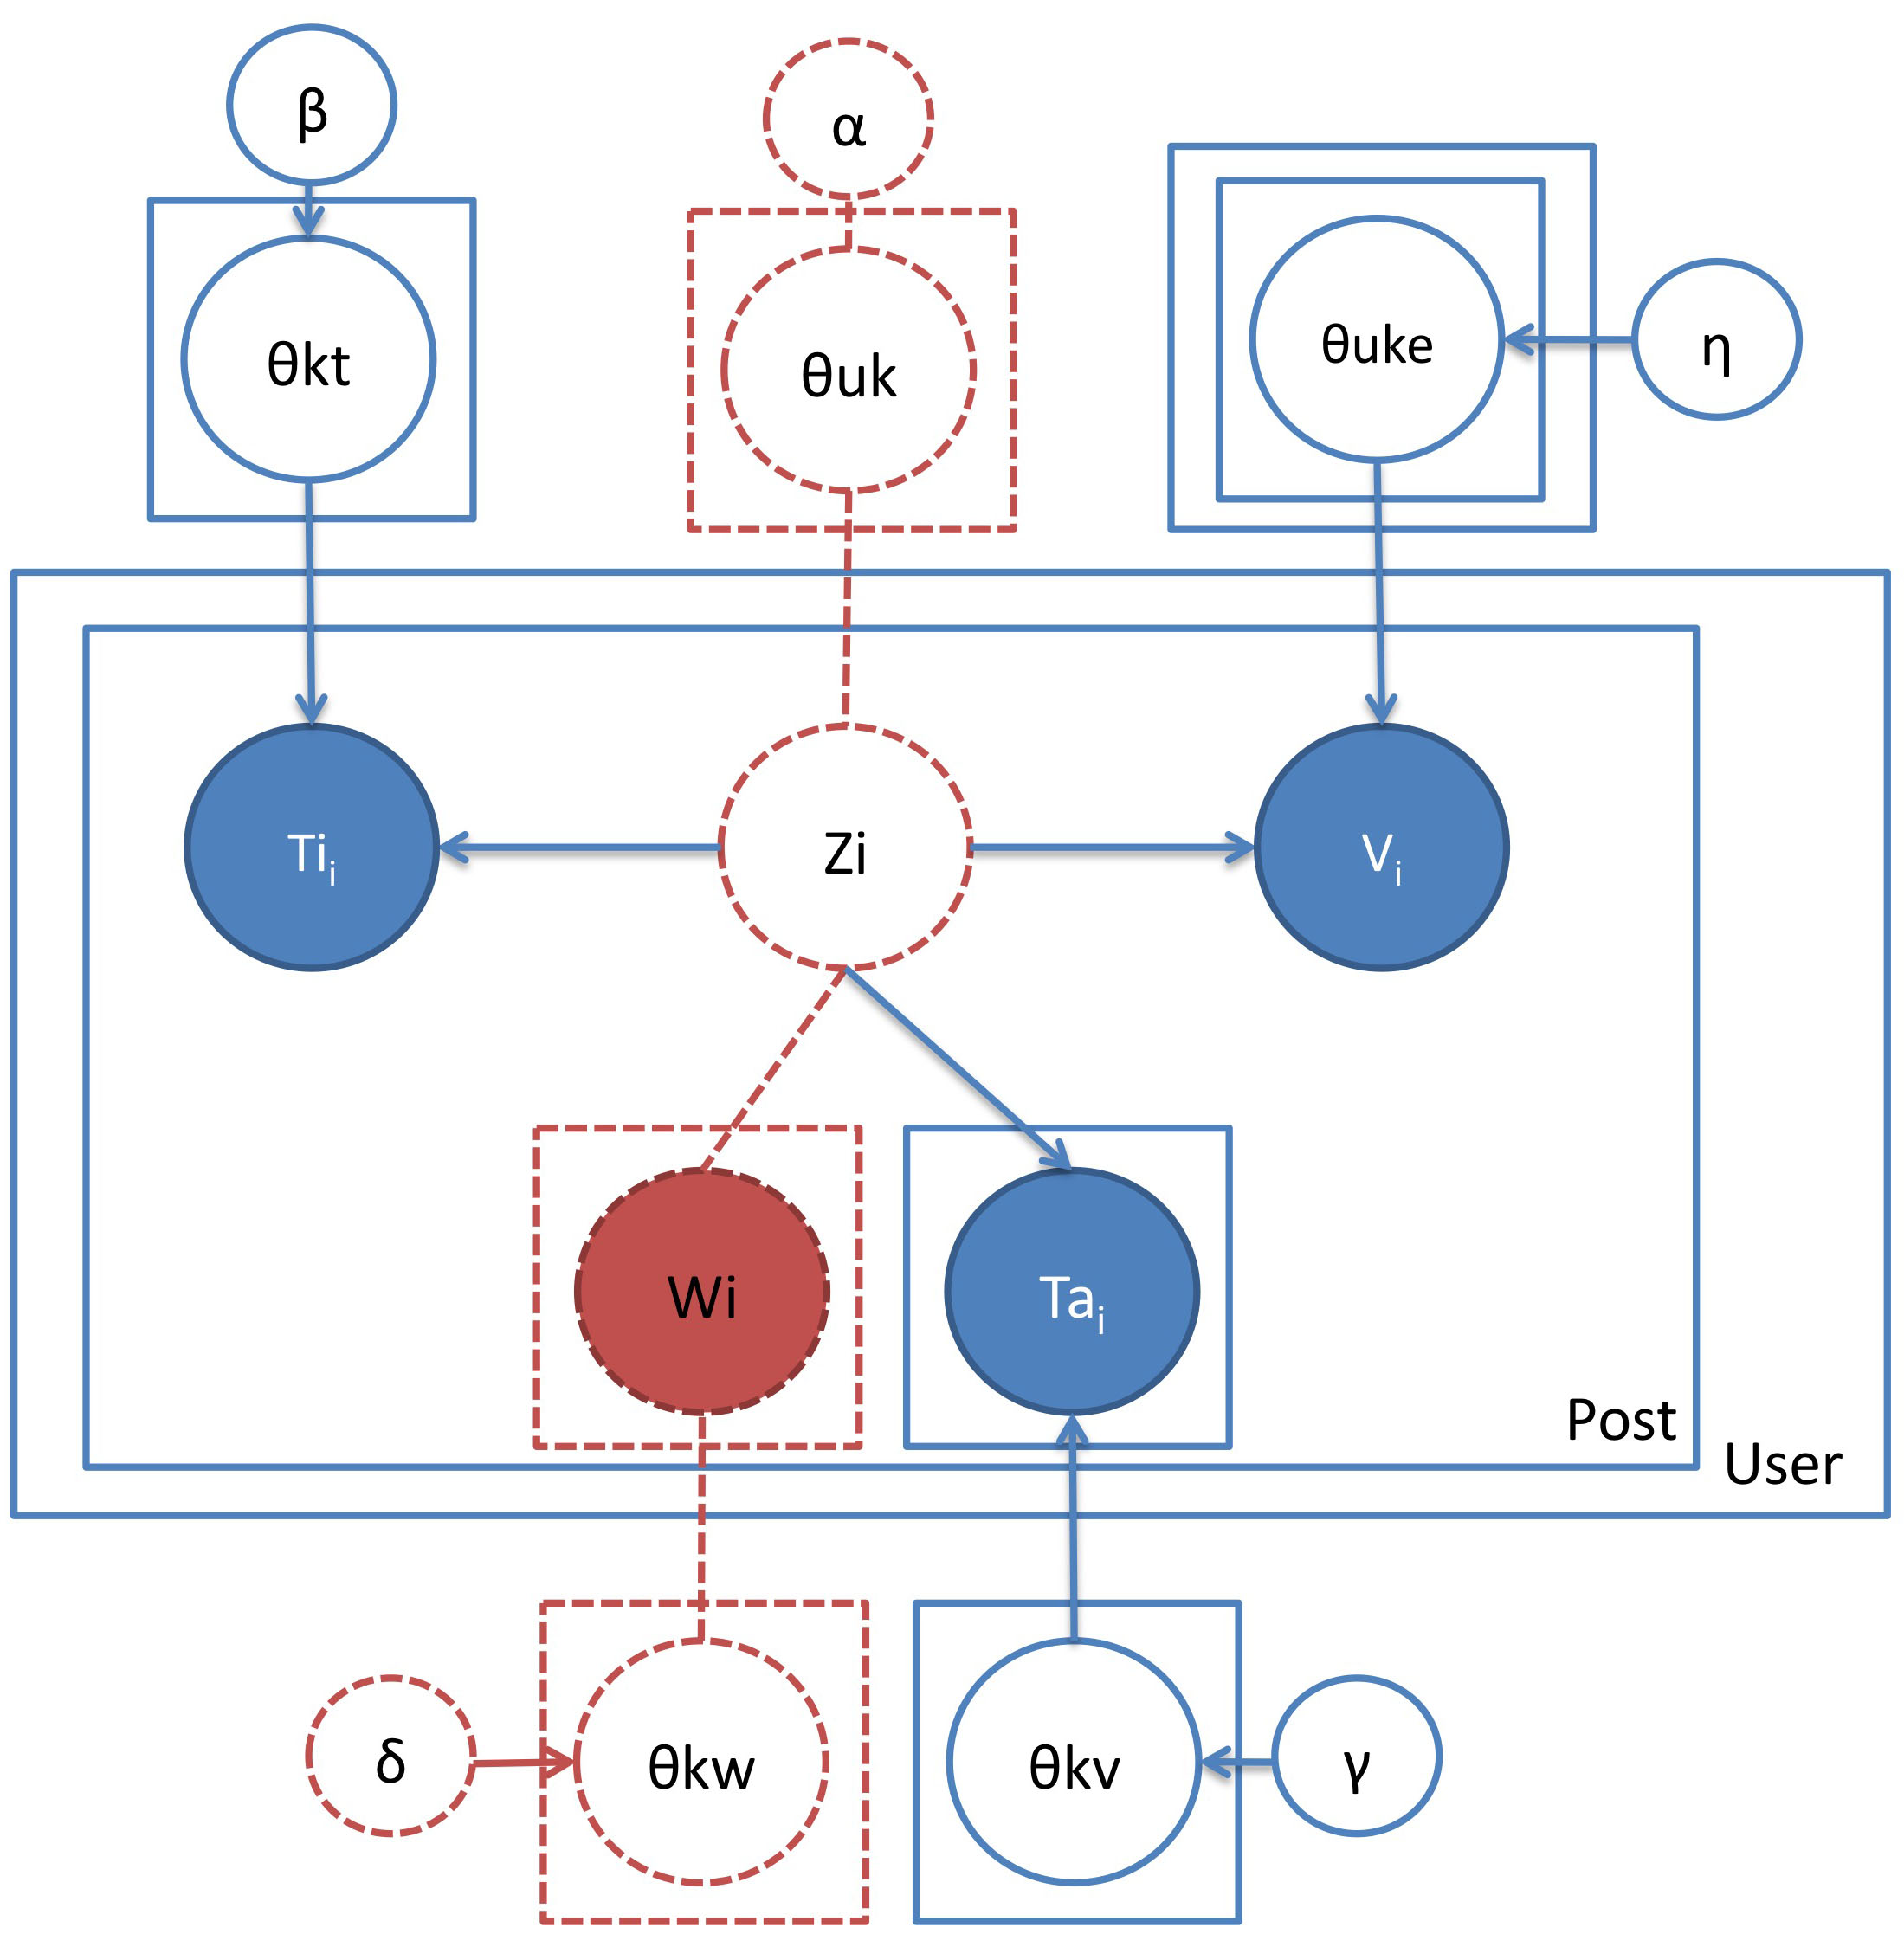
\includegraphics[ width=5.1in]{tteafinal.jpg}  
\caption{TTEA Model}
\label{fig:tteamodel} 
\end{figure}


Contrary to \cite{blei2003latent} who applied LDA model on long documents such as news articles and assumed that each word has a latent topic, we assume in TTEA that each answer post has one topic: like in other social media with short contributions, e.g. Twitter, an answer post is normally short, each answer post is therefore suitable to be assigned with one single latent topic, and all the words in that post are considered to be generated by this topic. Some work\cite{chp7zhao2011comparing}\cite{chp7diao2012finding} on microblog also made this assumptions.

For expertise modeling, we do not use votes directly because (a) the vote scores are sparse and noncontinuous, and (b) it is not reasonable to tell that a vote score $55$ is better than a vote score $50$ if the vote score are ranging from $0$ to $3000$.  Since the vote scores' counts distribution follows a log distribution\cite{yang2013cqarank}, we use the logarithmic value of vote score, and separate them into several expertise levels, which is one of the parameters: the expertise level.

For temporal modeling, like \cite{wang2006topics} \cite{hu2014user}, we use time stamps directly. In order to model time at different levels, we simply split time stamps into different parts (month, day, and hour) and use them separately depending on the demands.

%TODO in the following section some aspects have already been explained in previous chapters, you must at least indicate the aspects that remain the same and ifferentiate the new ones.
%DONE, this part is the description of generative process. It is not the same as problem define.

The generative process of TTEA model is :
Let us consider a user $u$ who wants to answer a question. She first selects a topic $k$ according to her user-topic distribution $\theta_{uk}$. Then she writes an answer post $p$. The words of $p$ are generated from topic $k$'s topic-word distribution $\theta_{kw}$. Since only the questions have tags, we consider the answers automatically acquire all the tags of the question they respond to. Then the answer post $p$ acquires its tags according to the topic-tag distribution $\theta_{kv}$ of topic $k$. Meanwhile, the answer post $p$ gets a time-stamp $ti$ according to the topic-time distribution $\theta_{kt}$ of topic $k$.
This procedure is described as follows,

%TODO: the following should be pseudo code in my opinion
%DONE

\begin{algorithm}%[htp]
\begin{algorithmic}[1]
\label{algo:algotopic}
\State \textit{/*The generative process*/}
\For { the u-th user $u$ \textbf{in} $U$ }
\State draw user topic distribution $\theta_{uk}$ $\sim$ Dir( $\alpha$) 
\EndFor
\For { the k-th topic $k$ \textbf{in} $K$ } 
\State draw topic tag distribution $\theta_{kv}$ $\sim$ Dir($\gamma$)
\State draw topic word distribution $\theta_{kw}$ $\sim$ Dir($\delta$)
\State draw topic time distribution $\theta_{kt}$ $\sim$ Dir($\beta$)
\EndFor
\For { the u-th user $u$ \textit{in} $U$ }
\For { the k-th topic $k$ \textit{in} $K$ }
\State draw user topic expertise distribution $\theta_{uke}$ $\sim$ Dir($\eta$) 
\EndFor
\EndFor
\For {the u-th user $u$ \textit{in} $U$}
\For {the n-th q\&a post $p$ \textit{in} $P$}
\State draw topic $z$ $\sim$ Multi($\theta_{uk}$)
\State draw time point $t$ $\sim$ Multi($\theta_{kt}$)
\State draw expertise level $v$ $\sim$ Multi($\theta_{uke}$) 
\For {the i-th word $w$ \textit{in} $W$ }
\State draw word $w$ $\sim$ Multi($\theta_{kw}$) 
\EndFor
\For {the j-th tag $ta$ \textit{in} $Ta$ } 
\State draw tag $t$ $\sim$ Multi($\theta_{kv}$)
\EndFor
\EndFor
\end{algorithmic}
\end{algorithm}

\subsection{TTEA Model Inference: using collapsed gibbs Sampling}

Like \cite{hu2014user}, we use the collapsed Gibbs Sampling algorithm \cite{griffiths2004finding} to sample the hidden variable $z$, based on which the unknown probabilities \{$\theta_{uk}$, $\theta_{kv}$, $\theta_{kw}$, $\theta_{kt}$,  and $\theta_{uke}$ \}%part of them, need to modified
can be estimated. % For simplicity we set the hyper parameters to \{$\alpha$, $\beta$, $\delta$, $\gamma$, $\eta$, $\lambda$\}.

%TODO cite the papers on how to tune the hyper parameters.
%DONE, this has been put into  the experiment.

%The TTEA inference process is as follows.
%We iteratively sample the topic indicator $z_i$ for each answer post $p_i$ according to equation \ref{eq:sample}. As explained before, each answer post will have one topic assignment. 

%TODO: why the following text is commented?
%DONE: has been moved to another subsection. 
%we sample the topic indicator z\_i for each answer post Ans\_i. Here we make the assumption that an Ans only has one topic. refer to paper (  Comprating twitter and traditional media using topic models.) 


%updated wi2016
The TTEA inference process is as follows.
We iteratively sample the topic indicator $z_i$ for each answer post $p_i$ according to equation \ref{eq:sample}. The intuition behind this equation is to combine two parts of possibilities: (1) the possibilities to generate the topic indicator $z_i$. (2) the possibilities generated by the topic indicator $z_i$. Besides, the intuition behind each part in Equation \ref{eq:sample} are corresponding to Equation \ref{eq:uk}, \ref{eq:kv}, \ref{eq:kw}, \ref{eq:kt} and \ref{eq:uke}. As explained before, each question/answer post will have one topic assignment. 


\begin{equation}
\begin{split}
p(z_i=k & | z_{\neg i}, \textbf{U}, \textbf{Ti}, \textbf{Ta}, \textbf{W}  ) \\
&\propto   \frac{ C_{u,\neg i}^k + \alpha_1 }{ \sum_{k=1}^K C_{u,\neg i}^k+ K* \alpha_1} \\
&\cdot \frac { \prod_{ta=1}^{Ta} \prod_{q=0}^{C_{ta}-1} ( C_{k,\neg i}^{ta} +q+\gamma) } { \prod_{p=0}^{\sum C_{ta} -1} \sum_{ta=1}^{Ta} (C_{k,\neg i}^v + p + Ta*\gamma  ) } \\
&\cdot \frac { \prod_{w=1}^{W} \prod_{s=0}^{C_w-1} ( C_{k,\neg i}^{w} +s+\delta) } { \prod_{t=0}^{\sum C_{w} -1} \sum_{w=1}^W (C_{k,\neg i}^w + t + W*\delta  ) } \\
&\cdot \frac{ C_{k,\neg i}^{ti} + \beta  }{\sum_{ti=1}^{Ti} C_{k,\neg i}^{ti} + Ti*\beta} \\
&\cdot \frac{ C_{u,k,\neg i}^{e} + \eta }{\sum_{e=1}^{E} C_{u,k,\neg i}^{e} + E * \eta}\\
\end{split}
\label{eq:sample}
\end{equation}

\noindent
where $\neg i$ enforces that all the counters used are calculated with the answer post $p_i$ excluded. $C_{u,\neg i}^k$ is the number of posts by user $u$ assigned to topic $k$, $C_{ta}$ is the number of tags $ta$ in $p_i$, therefore, $\sum C_{ta}$ is the total number of tags in $p_i$, $C_{k,\neg i}^{ta}$ is the number of tags $ta$ assigned to topic $k$. Similarly, $C_{w}$ is the number of words $w$ in $p_i$, $\sum C_{w}$ is the number of words in $p_i$, $C_{k,\neg i}^{w}$ is the number of words $w$ assigned to topic $k$. $C_{k,\neg i}^{ti}$ is the number of posts assigned to topic $k$ and posted at time $ti$. $C_{u,k,\neg i}^{e}$ is the number of posts which are assigned to topic $k$ and got a vote score in the range of expertise level $e$.

Then, with the result of the Gibbs sampling algorithm, we can make the following parameter estimation:
\begin{equation}\scriptsize
\theta_{uk}=\frac{ C_u^k + \alpha }{ \sum_{k=1}^K C_u^k+ K* \alpha} 
%\text{user-topic distribution}\\
\label{eq:uk}
\end{equation}
\begin{equation}\scriptsize
\theta_{kv}=\frac{ C_k^{ta} + \gamma }{ \sum_{ta=1}^{Ta} C_k^{ta}+ Ta* \gamma}
%\;\;\;\;\;\;\;\;\;\;\;\;\;\;\;\
%\text{topic-tag distribution}
\label{eq:kv}
\end{equation}
\begin{equation}\scriptsize
\theta_{kw}=\frac{ C_k^w + \delta }{ \sum_{w=1}^W C_k^w+ W* \delta}
%\;\;\;\;\;\;\;\;\;\;\;\;\;\;\;\
%\text{topic-word distribution}
\label{eq:kw}
\end{equation}
\begin{equation}\scriptsize
\theta_{kt}=\frac{ C_k^{ti} + \beta }{ \sum_{ti=1}^{Ti} C_k^{ti}+ Ti* \beta}
%\;\;\;\;\;\;\;\;\;\;\;\;\;\;\;
%\text{topic-time distribution}
\label{eq:kt}
\end{equation}
\begin{equation}\scriptsize
\theta_{uke}=\frac{ C_{u,k}^e + \eta }{ \sum_{e=1}^E C_{u,k}^e+ E* \eta} 
%\;\;\;\;\;\;\;\;\;\;\;\;\;\;\;
%\text{user-topic-expertise distribution}
\label{eq:uke}
\end{equation}


\subsection{Post Processing: Extracting activity indicators}\label{sec:detailed}

The previous model can only generate the distributions \{$\theta_{uk}$, $\theta_{kv}$, $\theta_{kw}$, $\theta_{kt}$, and $\theta_{uke}$ \}. To generate the other distributions, e.g. $\theta_{ku}$, $\theta_{tk}$ and $\theat_{ukt}$, we directly use the sample results at each iteration and keep recording the corresponding counters. Therefore, $C_k^u$ is the number of posts assigned to topic $k$ and posted by user $u$, $C_{ti}^k$ is the number of posts posted at time $ti$ and assigned to topic $k$. $C_{u,k}^{ti}$ is the number of posts by user $u$, assigned to topic $k$ and posted at time $ti$.
% $C_{u,k}^e$ is the number of posts by user $u$ assigned to topic $k$ with an expertise level $e$. We use the same method to estimate the probabilities.
Then, we estimate $\theta_{ku}$, $\theta_{tk}$, $\theat_{ukt}$ according to the following equations:
\begin{equation}%\scriptsize
\theta_{ku}=\frac{ C_k^u + \alpha_2 }{ \sum_{u=1}^U C_k^u+ U* \alpha_2} 
%\;\;\;\;\;\;\;\;\;\;\;\;\;\;\;\;\;\;\;\;\;\;\;\;\;\;
%\text{topic-user distribution}
\end{equation}
\begin{equation}%\scriptsize
\theta_{tk}=\frac{ C_{ti}^{k} + \beta_1 }{ \sum_{k=1}^{K} C_{ti}^{k}+ K* \beta_1}
%\;\;\;\;\;\;\;\;\;\;\;\;\;\;\;\;\;\;\;\;\;\;\;\;\;
%\text{time-topic distribution}
\end{equation}
\begin{equation}%\scriptsize
\theta_{ukt}=\frac{ C_{u,k}^{ti} + \lambda }{ \sum_{ti=1}^T C_{u,k}^{ti}+ T* \lambda} 
%%\;\;\;\;\;\;\;\;\;\;\;\;\;\;\;\;\;\;\;\;\;
%\text{user-topic-time distribution}
\end{equation}

%TODO: you have a lot of commented content in this section ; I saw that some definitions are indeed no longer used but check that them all to make sure you are not missing some details.
%DONE not use them anymore







\section{TTEA Experiments and Evaluation on StackOverflow data}\label{sec:TTEAexperiment}

\subsection{Basic statistic of StackOverflow Dataset: an overview}

%TODO do not repeat the part that was already described in previous chapter: make sure that each chapter only adds the new parts and always indicate the difference
%DONE,  new section 3.3
We conducted experiments on a dataset from StackOverflow. This site releases its whole content every three month. For our experiments, we used the data dump from July 2008 to March 2013. 

Table \ref{tab:basicinfo} and figure \ref{fig:basicstat} provide basic statistics on the dataset.
\begin{table}[htp]
\caption{Basic statistics on the dataset}
\label{tab:basicinfo}
\centering
\begin{tabular}{|c|c|}
\hline
number of tags & 32,379\\ \hline
number of questions & 4,592,961 \\ \hline
number of users asking questions & 833,041 \\ \hline
number of users providing answers & 8,585,113\\ \hline
number of questions having accepted answers & 2,808,825\\ \hline

\end{tabular}
\end{table}

\begin{figure}
\centering
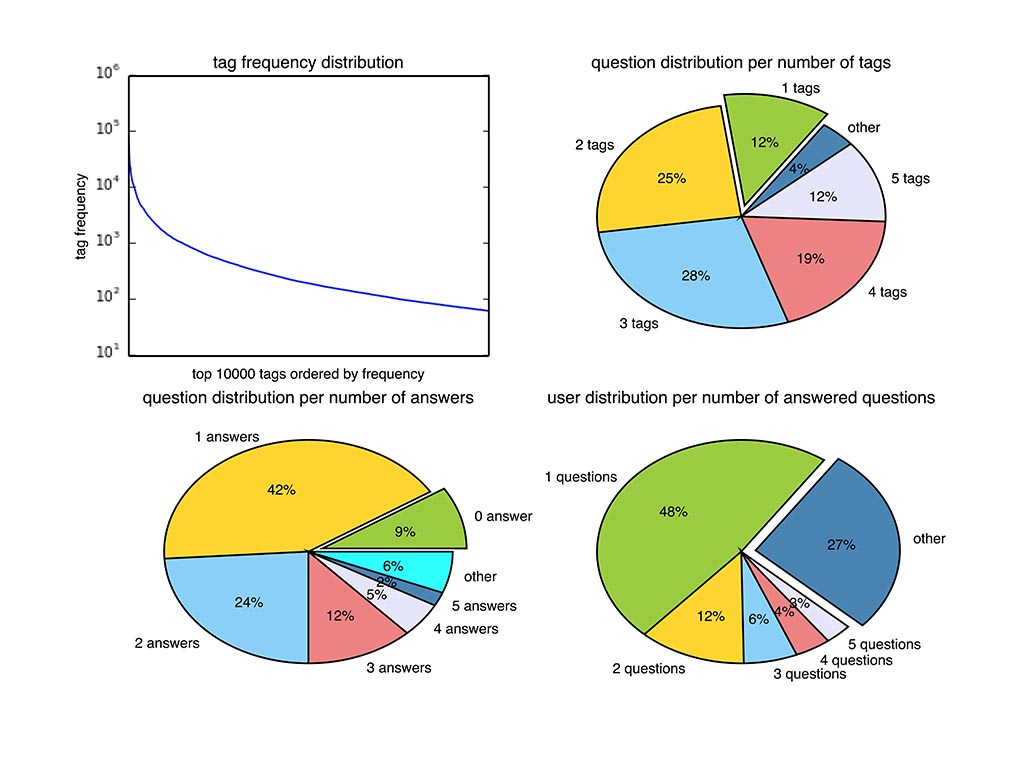
\includegraphics[ width=5in]{output.jpg}  
\caption{Basic perspectives of the dataset}
\label{fig:basicstat} 
\end{figure}

%TODO: include as many figures, charts, etc. as you can.
%fig: number of user answered questions.
%fig: number of user for each questions.
%fig: distribution of tags per questions.
%fig: tag frequency

%TBD
%fig: title_length vs num_answer. 
%fig: heatmap of question and answer. 
%

%TODO it seems to me that most of this should migrate to 5.2 TTD experiment on stackoverflow or if the datasets are differents you must idicate it and have the same details in each section, currently 5.2 does not have enough details
%DONE, dataset in 5.2 is mainly focus on the co-answer graph.

Here are some general observations about the dataset: 
\begin{itemize}
    \item nearly half of the questions do not have accepted answers;
    \item nearly half of the questions only have one answer and it maybe inadequate;
    \item more than a third of the questions only have one or two tags;
    \item nearly half of the users only answer one question so question routing and incentives are important problems;
    \item nearly 10\% percent of the questions do not have answers.
\end{itemize}


%TODO: some of this information is not specific to the introduction of time i.e. it is useful to LDA, TTD and TTEA and therefore it could be said before. One possibility is to create a section 3.3 before the suammary in section 3 dedicated to describing STack Overflow and the dump you will use for your evaluations in the other sections.
%DONE

\subsection{Experiment Dataset and Compared Methods}
In Chapter \ref{chap:ttd}, we only use a part of this data set (from 2008 to 2009), and we mainly focus on several co-answer graph. Besides, we also labeled this small dataset.
In this Chapter, due to the large volume of the dataset over 3 years, the processing time is extremely long. \cite{chp7ldatimecomplexity} shows that the complexity of each iteration of the Gibbs sampling for LDA is linear with the number of topic and the number of documents, which is $O(KN)$.   Since we are focusing on evaluate the effectiveness of our model, so in order to simplify the processing, for the following experiments, we chose two continuous months from the dataset (From Jan 2011 to June 2011, From July 2011 to Jan 2012), with no bias to the selections.% the period of selection will not lead any bias to the experiment.

%TODO: here you are raising concerns about scalability so you need to give details on the time it takes, complexity, etc.
%DONE, here we care more about effectiveness rather than efficiency. and explained the complexity for topic model.

%\subsection{Compared Methods: other probabilistic graphical model}

To evaluate the effectiveness of our model, we compared it with several related works:  
\begin{itemize}
\item{TTEA} is our method for modeling user, topic, temporal and expertise in Q\&A sites. Besides, we also model activities by adding virtual nodes. We can generate the user-topic distribution and topic-activity distribution simultaneously. 
\item{TEM}: \cite{yang2013cqarank} proposed a model for user, topic and expertise in Q\&A sites. It integrates a Gaussian Mixture Model to model expertise, which is time consuming. We simplify this process by directly modeling votes information. Besides, it does not model temporal information and user topic activities. 
\item{UQA}: \cite{guo2008tapping} proposed a User-Question-Answer model for modeling users and topics in Q\&A  sites. In certain Q\&A  sites, questions have category information which have proved to be very useful. The category in their model is similar to tags in TTEA model and TEM model. However we allow multiple tags for each posts while they can only set a single category.
\item{GrosToT}: \cite{hu2014user} proposed a User-Group-Topic-Time model for modeling users, groups, topics and time in social media sites. It introduces a group level between user and topic compared with other models. It does not directly generate user-topic distribution, so we compute it with the user-group distribution and group-topic distribution.% $\theta_{uk}$ so we compute it by $\theta_{uk} \propto \sum_{g=1}^{G} \theta_{ug} * \theta_{gk}$.
\item{LDA}: based on \cite{blei2003latent} we apply LDA model to create a User-Topic-Post model for modeling users and topics. It can generate the user-topic distribution and topic-words distribution.
%\begin{equation}\scriptsize
%\end{equation}

\end{itemize}

%TODO: the evaluation and its description must be different from the TTD one and emphize the time aspect that was added.
%DONE explained below.

We choose the same number of topics K=\textit{30} as \cite{Chang:2013} and the same number of expertises E=\textit{10} as \cite{yang2013cqarank}, which have proved to be a reasonable setting for the Stackoverflow dataset. We empirical set Dirichlet hyper parameters $\alpha_1$=$\alpha_2$=50/K, $\beta_1$=$\beta_2$=0.01, $\delta$=$\lambda$=$\eta$=0.01, $\gamma$=0.001 according to suggestions in \cite{griffiths2004finding}. 


\subsection{Performance of Topic Extraction: perplexity score}

%TODO: when you re-evaluate aspects common to TTD and TTEA you must explain why you redo it ; my understanding is that since you modified it you have to re-evaluate but even if this is the case you have to say it.
%DONE
In Chapter \ref{chap:ttd}, we have evaluated the perplexity score for both TTD and LDA model. The evaluation is to check if our model can have the same or better performance on topic extraction compared with much complicated probabilistic graphical model. In this section, we re-evaluate the perplexity score only among those probabilistic graphical models as our TTEA model is a probabilistic graphical model. Besides, we evaluate on a much larger dataset compared with Chapter \ref{chap:ttd}.

Table \ref{tab:toptagsp} and Table \ref{tab:topwordsp} show the top tags and words detected by our model. We use again the Perplexity~\cite{blei2003latent} metric as a quantitative way to measure the performance of topic extraction.

We include in our training dataset all the posts in the two months from August $1^{st}$ 2011 to October $1^{st}$ 2011, from users having more than 80 posts (as in \cite{yang2013cqarank}).
The resulting training dataset contains 87516 q\&a posts by 674 users. For data preprocessing, we tokenize text and removed the stop words. For the testing dataset, we use all the posts of the same set of users than the training data but this time from October $1^{th}$ 2011 to January $1^{th}$ 2012. So training and testing datasets have no overlap but concern the same community. We vary the number of topics: 10, 30, 50, and 100. 
For a testing set of M posts, $N_i$ denotes the number of words in the $i^{th}$ post and the Perplexity score is computed according to equation \ref{eq:getperplexity}.
%\begin{small}
\begin{equation} %\scriptsize
  Perplexity(D_{test})=exp\left\{-\frac{\sum_{i=1}^{M}\log p(W_i)}{\sum_{i=1}^{M}N_i}\right\}
\label{eq:getperplexity}
\end{equation}
%\end{small}
where $p(W_i)$ is the probability of the words in the test document $d_i$. In our model, $p(W_i)$ is computed according to equation \ref{eq:getprobabilitywords}.:% $P(W_i)=\sum_{k}\theta_{u_ik}\prod_{w} \theta_{kw_i}$:
\begin{equation}%\scriptsize
  P(W_i)=\sum_{k}\theta_{u_ik}\prod_{w} \theta_{kw_i}
\label{eq:getprobabilitywords}
\end{equation}
\begin{figure}[htp]
\centering
%\epsfig{file=fly.eps, height=1in, width=1in}
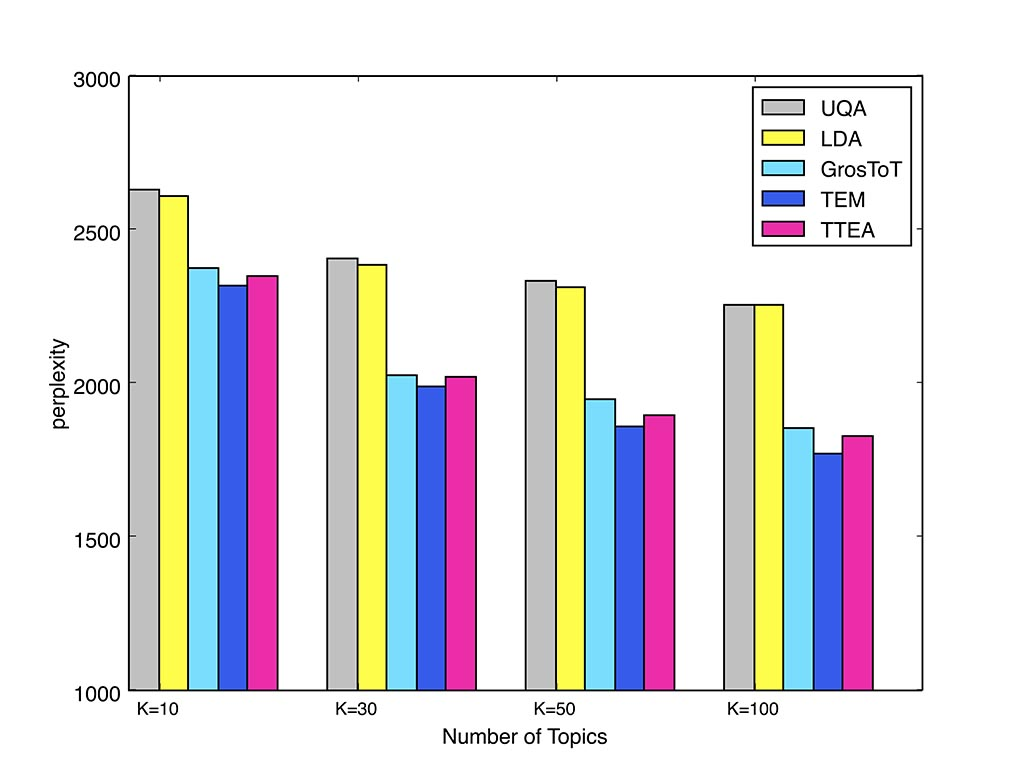
\includegraphics[width=5in]{perplexityv2.jpg}  % use this if you use "pdflatex"
\caption{Comparison of topic extraction performances}
\label{fig:perplexity} % Fig.2
\end{figure}



\begin{sidewaystable}
%\begin{table*}[htp]
%\begin{table}[!t]
\caption{Top tags for different topics generated by the TTEA model}
\label{tab:toptagsp}
\centering
\scriptsize
%\begin{tabular}{p{34pt}p{34pt}p{34pt}p{34pt}p{34pt}p{34pt}p{34pt}p{34pt}p{34pt}p{34pt}}
\begin{tabular}{cccccccccc}
\hline
Topic 1& Topic 2& Topic 3& Topic 4 & Topic 5 & Topic 6& Topic 7 & Topic 8 &Topic 9 & Topic 10\\
\hline
php&c#&iphone&c++&javascript&android&sql&java&jquery&git \\ 
xslt&.net&objective-c&c&jquery&java&mysql&spring&javascript&svn \\ 
xml&linq&ios&pointers&php&android-layout&sql-server&eclipse&html&version-control \\ 
xpath&generics&xcode&templates&ajax&listview&php&jsp&css&github \\ 
mysql&asp.net&cocoa-touch&stl&html&activity&query&.htaccess&jquery-selectors&mercurial \\ 
html&vb.net&ipad&arrays&json&android-intent&tsql&servlets&jquery-ui&eclipse \\ 
arrays&c#-4.0&uitableview&vector&asp.net&sqlite&sql-server-2008&jsf&dom&tortoisesvn \\ 
jquery&reflection&iphone-sdk-4.0&string&jquery-ajax&layout&join&mod-rewrite&php&linux \\ 
javascript&entity-framework&cocoa&function&forms&android-widget&select&maven&javascript-events&clearcase \\ 
foreach&list&xcode4&c++11&asp.net-mvc-3&xml&sql-server-2005&apache&ajax&ssh \\
\hline
\end{tabular}
%\end{table*}
\end{sidewaystable}

\begin{sidewaystable}
%\begin{table*}[htp]
%\begin{table}[!t]
\caption{Top words for different topics generated by the TTEA model}
\label{tab:topwordsp}
\centering
%\scriptsize
%\begin{tabular}{p{34pt}p{34pt}p{34pt}p{34pt}p{34pt}p{34pt}p{34pt}p{34pt}p{34pt}p{34pt}}
\begin{tabular}{cccccccccc}
\hline
Topic 1& Topic 2& Topic 3& Topic 4 & Topic 5 & Topic 6& Topic 7 & Topic 8 &Topic 9 & Topic 10\\
\hline
xsl&aspx&view&std&jquery&android&select&html&jquery&git \\ 
td&msdn&reference&const&ajax&activity&join&java&div&branch \\ 
tr&microsoft&nsstring&pointer&script&html&group&file&click&commit \\ 
template&library&apple&char&javascript&view&order&spring&element&file \\ 
select&select&html&template&page&developer&table&jar&event&svn \\ 
row&linq&library&vector&html&intent&key&apache&input&repo \\ 
echo&system&documentation&operator&form&reference&count&eclipse&document&repository \\ 
table&dictionary&developer&compiler&url&layout&row&docs&text&files \\ 
match&ienumerable&ios&memory&document&try&inner&servlet&html&master \\ 
node&expression&release&struct&json&button&query&web&api&github \\ 
\hline
\end{tabular}
%\end{table*}
\end{sidewaystable}

Figure \ref{fig:perplexity} shows the perplexity results for our TTEA method and other state-of-the-art methods. %We compare to 
TTEA is almost as good as TEM. But TEM integrates a Gaussian Mixture Model, which is time consuming. The training process of TEM is nearly three times longer than the other models.





\subsection{Question Routing: recommend new question to potential users}
\label{sec:qrouting}
\cite{Chang09} suggested that topic models should focus on evaluations on real-world task performance rather than on optimizing likelihood-based measures. So, in addition to the perplexity-based evaluation, we used the results of TTEA to perform real-word tasks and we evaluated them. This is described in the following subsections.
Given a question $q$ and a set of users $U$, the task is to rank all these users by their interests to answer question $q$.
We score each user $u$ by considering the similarity between his topics of interest and the topics of the question ($Sim(u,q)$). The intuition behind equation \ref{eq:simquestion} is that the more a user is interested in the topic of a question, the more likely he is to provide an answer to that question.
\begin{equation}
Sim(u,q) = (1 -JS(\theta_{uk},\theta_{qk}))
\label{eq:simquestion}
\end{equation}
where $\theta_{uk}$ is the user topic interest distribution, $\theta_{qk}$ is the question topic distribution, and JS(.) is the Jensen–Shannon divergence distance. We obtain $\theta_{uk}$ directly from model results. For $\theta_{qk}$, we apply equation \ref{eq:thetaqk}.
\begin{equation}
\begin{split}
\theta{q,k} &\propto p(k|w_q,t_q,u) \\
           &=p(k|u)p(w_q|k)p(t_q|k) \\
           &= \theta{uk} \sum_{w_i \in w_q} \theta_{kw_i} \sum_{t_i \in t_q} \theta_{kv_i} 
\end{split}
\label{eq:thetaqk}
\end{equation}
where $w_q$ and $t_q$ are the sets of all the words and tags in question $q$ and $\theta{kw}$, $\theta{kv}$ are the topic-word distribution and topic-tag distribution obtained directly from the model result. Then for question $q$, we compute the $Sim$ score for user set $U$ and rank them in decreasing order. % of the $Sim$ score.


We used all the posts from July $1^{th}$ 2011 to October $1^{th}$ 2011 from users having more than 50 q\&a posts for the training dataset. Rather than using thethreshold of 80 post like in \cite{yang2013cqarank}, we empirically set it to 50 posts to get enough users for recommendation. 
The resulting training set contains 297881 posts by 2555 users. For the testing dataset, we use all the questions posted by the same set of users as in the training set but this time from October $1^{th}$ 2011 to January $1^{th}$ 2012. Therefore the training and testing datasets have no overlaps. We removed testing questions which have no, or only one, answer. The resulting test dataset contains 6044 questions, 18077 answers and 7888 involved users. 

We also chose another period for this experiment. Besides, we vary the number of topics by $15$ and $50$, we vary the filter limit by $40$ and $80$. These experimental results are shown in section \ref{sec:parasetting}.

In order to evaluate different models, we consider precision at position N ( Precision@N or simply P@N) and recall at position N (Recal@N or simply R@N), which are widely used measures in the Information Retrieval community. Let $R_q$ be the recommendations of users for a question $q$ and $U_q$ be the actual set of users who posted for question $q$. Then Precision@N is defined in equation \ref{eq:precisionatn} and Recal@N is defined in equation \ref{eq:recallatn}.
\begin{equation}%\scriptsize
 P@N = \frac{1}{|Q|}\sum_{q \in Q}\frac{|R_q \cap U_q|}{|R_q|}
\label{eq:precisionatn}
 \end{equation}
 
 \begin{equation}%\scriptsize
 R@N = \frac{1}{|Q|}\sum_{q \in Q}\frac{|R_q \cap U_q|}{|U_q|}
\label{eq:recallatn}
 \end{equation}

\noindent
where $Q$ is the set of testing questions. Like in \cite{Chang:2013}, we use the Matching Set Count (MSC)  
which is defined in equation \ref{eq:matchingsetcount}. The idea is to count the number of successful recommendations, i.e., for which at least one of the recommended users answered the question.
 \begin{equation}%\scriptsize
 MSC@N = \frac{1}{|Q|}\sum_{q \in Q} 1[R_q \cap U_q \neq \emptyset]
\label{eq:matchingsetcount}
 \end{equation}
 where $1[condition]$ is equal to 1 if $condition$ is true, otherwise 0. 

\begin{sidewaystable}
% \begin{table*}[htp]
\caption{Question Routing experiments, Random denotes that we randomly recommend users for the test questions.}
\label{tab:qrouting}
%\scriptsize
\centering
\begin{tabular}{|c|c|c|c|c|c|c|c|c|c|c|c|c|}
\hline
 & p@5    &p@10    &p@20   & p@30 &r@5 & r@10 & r@20 &r@30 & msc@5 & msc@10 &msc @20 &msc@30  \\ \hline


%average 5 times, 
TTEA&0.024&0.019&0.015&0.013&0.045&0.072&0.111&0.142&0.112&0.178&0.269&0.339 \\ \hline
TTEA-ACT&0.028&\textbf{0.022}&\textbf{0.017}&\textbf{0.014}&0.052&\textbf{0.083}&\textbf{0.127}&\textbf{0.159}&0.134&\textbf{0.209}&\textbf{0.313}&\textbf{0.382} \\ \hline
TEM&0.024&0.019&0.015&0.013&0.045&0.073&0.114&0.146&0.114&0.179&0.275&0.344 \\ \hline
TEM-ACT&0.029&\textbf{0.023}&\textbf{0.018}&\textbf{0.015}&0.054&\textbf{0.084}&\textbf{0.129}&\textbf{0.162}&0.137&\textbf{0.210}&\textbf{0.315}&\textbf{0.388} \\ \hline
UQA&\textbf{0.030}&0.019&0.012&0.010&\textbf{0.062}&0.075&0.095&0.112&\textbf{0.149}&0.179&0.224&0.261 \\ \hline
GROSTOT&0.027&0.017&0.011&0.009&0.055&0.067&0.085&0.099&0.134&0.164&0.204&0.236 \\ \hline
RANDOM&0.001&0.001&0.001&0.001&0.001&0.002&0.005&0.007&0.003&0.007&0.013&0.019 \\ \hline
\end{tabular}
%\end{table*}
\end{sidewaystable}

In addition, our model can capture activity and we believe this information improves question routing. The intuition is that even if a user has a high $Sim$ score for a question, the less he is active, the less likely he is to provide an answer to that question. Therefore, we define a score $SimAct$ to combine both topic similarity and activity level as shown in equation \ref{eq:newscore}, where $Act(u,q)$ is the computed activity score for user $u$ to question $q$. A high value of the $Act$ score indicates a high probability of activity on a question. We use TTEA to denote the method using only the similarity information, that is to say, ranking users by $Sim$ score. We use TTEA-ACT to denote the method using both similarity and activity, that is to say, ranking users by $SimAct$ score. We also integrated our activity model to the TEM model  and we refer to it as TEM-ACT. 
\begin{equation}
\begin{split}
SimAct(u,q) &= (1 -JS(\theta_{uk},\theta_{qk}))* Act(u,q) \\
         &= (1 -JS(\theta_{uk},\theta_{qk}))* \sum_{k=1}^{K} \theta_{qk} * \theta_{ku}
\end{split}
\label{eq:newscore}
\end{equation} 

%TODO search all the text in your thesis en replace (1)... (2)... by real latex number lists since you have no space constraint in the thesis.
%DONE 

Table \ref{tab:qrouting} shows the results. We ran the experiments five times and listed the average scores. Our observations can be summerized as follows:
\begin{itemize}
    \item UQA and GROSTOT perform the better when the number of recommended users are small, and TTEA and TEM begin to outperform UQA and GROSTOT when the number of recommended users is large;
    \item TTEA-ACT shows the best performances compared with the baseline competitors;
    \item both TTEA-ACT and TEM-ACT perform better than the other models. The activity modeling is a generic method that could improve the performance not only of our model, but also of other models although here we only show the result for the activity model with TEM as an example;
    \item even if TEM or TEM-ACT perform better than our model they remain again time consuming. Experiments show that the training process takes around 3$\sim$4 times longer compared to our model
\end{itemize}   


\subsection{Experiment Parameter Sensitivity Analysis}
\label{sec:parasetting}
For the training dataset, we used all the posts in a three months period, from January $1^{th}$ 2011 to March $31^{th}$ 2011, from users having at least 50 q\&a posts, rather than 80 posts like \cite{yang2013cqarank}, in order to get enough users for recommendations. The training set contains 371181 posts by 3123 users. For the testing dataset, we used all the questions posted by the same set of users as in the training set, but this time from April $1^{th}$ 2011 to June $31^{th}$ 2011. Therefore the training and testing datasets have no overlaps. We removed questions with no or only one answer. The resulting test dataset contains 9048 questions, 27870 answers and 10147 users. 
Table \ref{tab:qrouting123456} shows the question routing results. We can still find that TTEA-ACT outperforms all the baseline models. Besides, Both TTEA-ACT and TEM-ACT outperform all the other models. 

\begin{sidewaystable}
%\begin{table*}
\caption{Question Routing Experiments on Another Dataset}
\label{tab:qrouting123456}
%\scriptsize
\centering
\begin{tabular}{|c|c|c|c|c|c|c|c|c|c|c|c|c|}
\hline
 & p@5    &p@10    &p@20   & p@30 &r@5 & r@10 & r@20 &r@30 & msc@5 & msc@10 &msc @20 &msc@30  \\ \hline
TTEA&0.026&0.020&0.015&0.013&0.047&0.073&0.110&0.136&0.123&0.186&0.273&0.332 \\ \hline
TTEA-ACT&\textbf{0.032}&\textbf{0.026}&\textbf{0.019}&\textbf{0.016}&\textbf{0.058}&\textbf{0.093}&\textbf{0.137}&\textbf{0.168}&\textbf{0.153}&\textbf{0.236}&\textbf{0.339}&\textbf{0.405} \\ \hline
TEM&0.025&0.021&0.016&0.013&0.047&0.076&0.112&0.139&0.120&0.191&0.274&0.333 \\ \hline
TEM-ACT&\textbf{0.032}&\textbf{0.025}&\textbf{0.020}&\textbf{0.016}&\textbf{0.058}&\textbf{0.092}&\textbf{0.141}&\textbf{0.171}&\textbf{0.153}&\textbf{0.235}&\textbf{0.348}&\textbf{0.411} \\ \hline
UQA&0.027&0.016&0.011&0.009&0.052&0.062&0.080&0.096&0.130&0.155&0.196&0.233 \\ \hline
GROSTOT&0.023&0.014&0.009&0.007&0.044&0.055&0.069&0.081&0.112&0.137&0.172&0.200 \\ \hline
RANDOM&0.001&0.001&0.001&0.001&0.001&0.002&0.004&0.005&0.003&0.005&0.010&0.015 \\ \hline
\end{tabular}
%\end{table*}
\end{sidewaystable}


Table \ref{tab:qroutingtop15} shows the question routing results with a number of topics set to 15. We use the same training and testing datasets as in section \ref{sec:qrouting}.

\begin{sidewaystable}
%\begin{table*}
\caption{Question Routing experiments with 15 topics}
\label{tab:qroutingtop15}
%\scriptsize
\centering
\begin{tabular}{|c|c|c|c|c|c|c|c|c|c|c|c|c|}
\hline
 & p@5    &p@10    &p@20   & p@30 &r@5 & r@10 & r@20 &r@30 & msc@5 & msc@10 &msc @20 &msc@30  \\ \hline
TTEA&0.016&0.013&0.012&0.010&0.030&0.050&0.086&0.112&0.076&0.127&0.213&0.269 \\ \hline
TTEA-ACT&0.023&\textbf{0.018}&\textbf{0.015}&\textbf{0.012}&0.042&\textbf{0.066}&\textbf{0.107}&\textbf{0.134}&\textbf{0.112}&\textbf{0.170}&\textbf{0.268}&\textbf{0.329} \\ \hline
TEM&0.017&0.015&0.012&0.010&0.032&0.054&0.091&0.115&0.083&0.137&0.222&0.276 \\ \hline
TEM-ACT&0.024&\textbf{0.018}&\textbf{0.014}&\textbf{0.012}&0.043&\textbf{0.068}&\textbf{0.103}&\textbf{0.131}&\textbf{0.114}&\textbf{0.172}&\textbf{0.254}&\textbf{0.319} \\ \hline
UQA&\textbf{0.028}&0.016&0.011&0.008&\textbf{0.056}&\textbf{0.066}&0.083&0.099&0.137&0.159&0.199&0.238 \\ \hline
Grostot&0.023&0.015&0.010&0.008&0.045&0.058&0.075&0.089&0.112&0.143&0.183&0.216 \\ \hline
Random&0.001&0.001&0.001&0.001&0.002&0.003&0.004&0.006&0.005&0.008&0.012&0.017 \\ \hline
\end{tabular}
%\end{table*}
\end{sidewaystable}

Table \ref{tab:qroutingtop50} shows the question routing results for the number of topics set to 50. We use the same training and testing datasets as in section \ref{sec:qrouting}.


\begin{sidewaystable}
%\begin{table*}
\caption{Question Routing experiments with 50 topics}
\label{tab:qroutingtop50}
%\scriptsize
\centering
\begin{tabular}{|c|c|c|c|c|c|c|c|c|c|c|c|c|}
\hline
 & p@5    &p@10    &p@20   & p@30 &r@5 & r@10 & r@20 &r@30 & msc@5 & msc@10 &msc @20 &msc@30  \\ \hline
TTEA&0.028&0.023&0.018&0.015&0.054&0.087&0.132&0.168&0.134&0.215&0.319&0.394 \\ \hline
TTEA-ACT&\textbf{0.033}&\textbf{0.025}&\textbf{0.019}&\textbf{0.016}&0.063&\textbf{0.095}&\textbf{0.142}&\textbf{0.178}&\textbf{0.158}&\textbf{0.235}&\textbf{0.343}&\textbf{0.418} \\ \hline
TEM&0.029&0.024&0.018&0.015&0.056&0.088&0.136&0.171&0.141&0.220&0.325&0.400 \\ \hline
TEM-ACT&\textbf{0.033}&\textbf{0.026}&\textbf{0.020}&\textbf{0.017}&0.062&\textbf{0.096}&\textbf{0.145}&\textbf{0.182}&\textbf{0.157}&\textbf{0.240}&\textbf{0.347}&\textbf{0.427} \\ \hline
UQA&0.032&0.019&0.012&0.010&\textbf{0.065}&0.077&0.097&0.116&\textbf{0.158}&0.185&0.227&0.270 \\ \hline
Grostot&0.028&0.017&0.011&0.009&0.056&0.067&0.088&0.102&0.136&0.163&0.210&0.241 \\ \hline
Random&0.001&0.001&0.001&0.001&0.002&0.002&0.005&0.007&0.004&0.006&0.013&0.018 \\ \hline
\end{tabular}
%\end{table*}
\end{sidewaystable}


Table \ref{tab:qroutingfilter40} shows the question routing results whith users having more than 40 posts. We use the same period of dataset used in section \ref{sec:qrouting}. Due to the different filter limit, the training set contains $3457$ users and $338485$ q\&a posts, the testing set contains $8579$ questions, $25500$ answers and $10135$ involved users.

\begin{sidewaystable}
%\begin{table*}
\caption{Question Routing experiments, with users having more than 40 posts}
\label{tab:qroutingfilter40}
%\scriptsize
\centering
\begin{tabular}{|c|c|c|c|c|c|c|c|c|c|c|c|c|}
\hline
 & p@5    &p@10    &p@20   & p@30 &r@5 & r@10 & r@20 &r@30 & msc@5 & msc@10 &msc @20 &msc@30  \\ \hline
TTEA&0.021&0.018&0.014&0.012&0.040&0.067&0.104&0.132&0.100&0.167&0.253&0.313 \\ \hline
TTEA-ACT&0.026&\textbf{0.021}&\textbf{0.016}&\textbf{0.014}&0.049&\textbf{0.076}&\textbf{0.118}&\textbf{0.149}&0.126&\textbf{0.193}&\textbf{0.292}&\textbf{0.360} \\ \hline
TEM&0.023&0.018&0.014&0.012&0.043&0.069&0.106&0.137&0.109&0.170&0.255&0.323 \\ \hline
TEM-ACT&0.027&\textbf{0.021}&\textbf{0.016}&\textbf{0.014}&0.050&\textbf{0.078}&\textbf{0.121}&\textbf{0.152}&0.128&\textbf{0.194}&\textbf{0.295}&\textbf{0.362} \\ \hline
UQA&\textbf{0.029}&0.018&0.011&0.009&\textbf{0.059}&0.071&0.087&0.101&\textbf{0.142}&0.169&0.205&0.235 \\ \hline
Grostot&0.025&0.016&0.010&0.008&0.050&0.063&0.077&0.091&0.122&0.152&0.188&0.217 \\ \hline
Random&0.000&0.000&0.000&0.000&0.001&0.002&0.003&0.005&0.002&0.004&0.008&0.013 \\ \hline
\end{tabular}
%\end{table*}
\end{sidewaystable}


Table \ref{tab:qroutingfilter80} shows the question routing results with users having more than 80 posts. We use the same period of dataset used in section \ref{sec:qrouting}. Due to the different filter limit, the training set contains $1275$ users and $216940$ q\&a posts, the testing set contains $2589$ questions, $8006$ answers and $4196$ involved users.
\begin{sidewaystable}
%\begin{table*}
\caption{Question Routing experiments,  with users having more than 80 posts}
\label{tab:qroutingfilter80}
%\scriptsize
\centering
\begin{tabular}{|c|c|c|c|c|c|c|c|c|c|c|c|c|}
\hline
 & p@5    &p@10    &p@20   & p@30 &r@5 & r@10 & r@20 &r@30 & msc@5 & msc@10 &msc @20 &msc@30  \\ \hline
TTEA&0.028&0.023&0.019&0.016&0.051&0.083&0.135&0.175&0.132&0.212&0.336&0.424 \\ \hline
TTEA-ACT&0.031&\textbf{0.026}&\textbf{0.020}&\textbf{0.018}&0.058&\textbf{0.094}&\textbf{0.146}&\textbf{0.188}&0.150&\textbf{0.238}&\textbf{0.364}&\textbf{0.457} \\ \hline
TEM&0.031&0.026&0.020&0.017&0.056&0.095&0.147&0.188&0.143&0.238&0.356&0.445 \\ \hline
TEM-ACT&0.035&\textbf{0.027}&\textbf{0.021}&\textbf{0.018}&0.063&\textbf{0.100}&\textbf{0.151}&\textbf{0.193}&0.165  &\textbf{0.253}&\textbf{0.375}&\textbf{0.468} \\ \hline
UQA&\textbf{0.040}&0.025&0.016&0.013&\textbf{0.077}&0.096&0.124&0.150&\textbf{0.194}&0.237&0.299&0.357 \\ \hline
Grostot&0.036&0.022&0.015&0.012&0.070&0.086&0.114&0.135&0.177&0.214&0.278&0.325 \\ \hline
Random&0.001&0.001&0.001&0.001&0.002&0.003&0.006&0.011&0.005&0.008&0.019&0.030 \\ \hline
\end{tabular}
%\end{table*}
\end{sidewaystable}

%TODO: you must conclude with a paragraph actually discussing the topic of this section: the Parameter Sensitivity
%done: conclude in the end of this section.

From the above experiments, we could found that our model with activity modeling also have consistent best performance on another period of time dataset. The performance increase when the topic number increase. This is because when topic number increase, the words in a topic are more concentrated. But there is also another problem when topic number parameter increase, which many generated topics are actually very similar. And increasing the topic number parameter will increase the execute time. The performance increase when we keep more active user by increasing filter threshold, which is the number of post a user has. There will be more active user as the question routing candidates.




%TODO: personnaly I believe evrytime you can you should generate a chart to visulize the tables in addition to giving the tables ; everytime you can you should give both. This applies to your entire thesis document. 
%TBD



\subsection{Recommendation of Expert Users: topic based expertise}
%\cite{yang2013cqarank}
Given a question $q$ and a set of users $U$, the task is now to recommend $N$ users until one of the users gets the highest vote. The point is to rank recommended users by their expertise to answer question $q$.
We score each user $u$ by considering the similarity $SimExp(u,q)$ between user topic interest and user topic expertise to answer question $q$. The intuition behind equation \ref{eq:simexpscore} is that if the user is interested in the question, she will probably provide an answer to that question and if the user has expertise on the question, the answer will probably have the highest vote score. 
\begin{equation}
SimExp(u,q) = (1 -JS(\theta_{uk},\theta_{qk}))* Exp(u,q)
\label{eq:simexpscore}
\end{equation}
where $\theta_{uk}$, $\theta_{qk}$ is the same than in \ref{eq:simquestion} for user topic interest distribution. For our method, we compute $Exp(u,q)$ by equation \ref{eq:computeEXP}
\begin{equation}
Exp(u,q) =  \sum_{e=1}^{E} \theta_{kue} * e
\label{eq:computeEXP}
\end{equation}
As UQA and GROSTOT do not model expertise, like \cite{yang2013cqarank}, we set $Exp(u,q)$ to 1 for these two methods. For TEM, we reuse equation \ref{eq:temexp} indicated in \cite{yang2013cqarank}.
\begin{equation}
Exp(u,q) =  \sum_{e=1}^{E} \phi_{z,u,e}* \mu_e
\label{eq:temexp}
\end{equation}


In order to evaluate different models, we consider the percentage of successful expert recommendation until position N. A successful expert recommendation until position N means that the N-th user, recommended by an algorithm, not only answers the question but also gets the highest votes. 


\begin{table}[htp]
\caption{Expert recommendation experiments}
\label{tab:expertrec}
%\scriptsize
\centering
\begin{tabular}{|c|c|c|c|}
\hline
Methods& N=30 & N=60 & N=100 \\ \hline
TEM&0.128&\textbf{0.228}&0.392 \\ \hline
TTEA&0.079&0.195&\textbf{0.443} \\ \hline
UQA&\textbf{0.146}&0.206&0.261 \\ \hline
Grostt&0.127&0.172&0.220 \\ \hline
Random&0.008&0.018&0.028 \\ \hline
\end{tabular}
\end{table}

Table \ref{tab:expertrec} shows the results. Random denotes a method where we randomly recommend users for the test questions. We ran the experiments five times and listed the average scores. We summarize our observations as follows: (1) Our TTEA shows the best performances compared with the baseline models when the number of recommended users is large. This means that when we recommend 100 users for each testing questions, in around $44\%$ cases we have one user not only answering the question, but also winning the highest vote. (2) When the number of recommended users is large, both TEM and TTEA perform better than other models which do not model expertise, so expertise modeling can improve expert recommendation. (3) TEM uses Gaussian Mixture Model to model expertise, while we directly model votes which is less precise. Therefore, we perform badly when the number of recommended users is small. (4) After ranking users by topic similarity scores, using expertise scores to re-rank those users actually lowers the probability of the top ranked user to answer the question. The intuition behind is that a user having high expertise on a question does not necessarily have high topic similarity score with the question.

\subsection{Trends: temporal dynamics at different levels}
With the temporal modeling of TTEA, we can explore topic dynamics at many different levels. We present illustrative case studies to show the advantage of temporal modeling.

We first set the time window at the month level. Figure \ref{fig:timelevel}-a shows the dynamics of $Android$, $Iphone$ and $Flash$ related topics at different months from Jan 2011 to Dec 2011. $Flash$ related topics are more active in the early of 2011, but become less popular in the late of 2011. We then set the time window at the day level. Figure \ref{fig:timelevel}-b shows the dynamics of $Android$, $Iphone$ and $Flash$ related topics from July $1^{st}$ 2011 to July $31^{st}$ 2011. We can see that all topics are active from Monday to Friday, and not active during the weekend. Lastly, we set the time window at the hour level. Figure \ref{fig:timelevel}-c shows the  dynamicsof  $Android$, $Iphone$ and $Flash$ related topics at different hours during a day. We can verify that both $Android$ and $Iphone$ related topics are more active during daytime, but $Flash$ related topics are more active during the afternoon.

Previous figures show the topic dynamics on a global level. We now illustrate the topic dynamics at the user level. We choose top active users according to the output of $\theta_{ku}$ in $Android$ related topic and $Iphone$ related topic separately. Figure \ref{fig:usertimelevel}-a,b show the activity pattern of the two most active users in $Iphone$ related topic. We can observe that the user in Figure \ref{fig:usertimelevel}-a is only active during work-time. The user seldom answers questions after 7PM. On the contrary, the user in Figure \ref{fig:usertimelevel}-b is active until very late but not midnight. Figure \ref{fig:usertimelevel}-c,d show the activity pattern of the two most active users in $Android$ related topic. We can observe that the user in Figure \ref{fig:usertimelevel}-c is active in the morning, afternoon and evening. On the contrary, the user in Figure \ref{fig:usertimelevel}-d is even active at midnight. For all these users, we can observe that they are not actually active on the topics they are not interested in. 
We believe this information will benefit many community management related tasks.

%left lower right upper
\begin{figure}
\centering
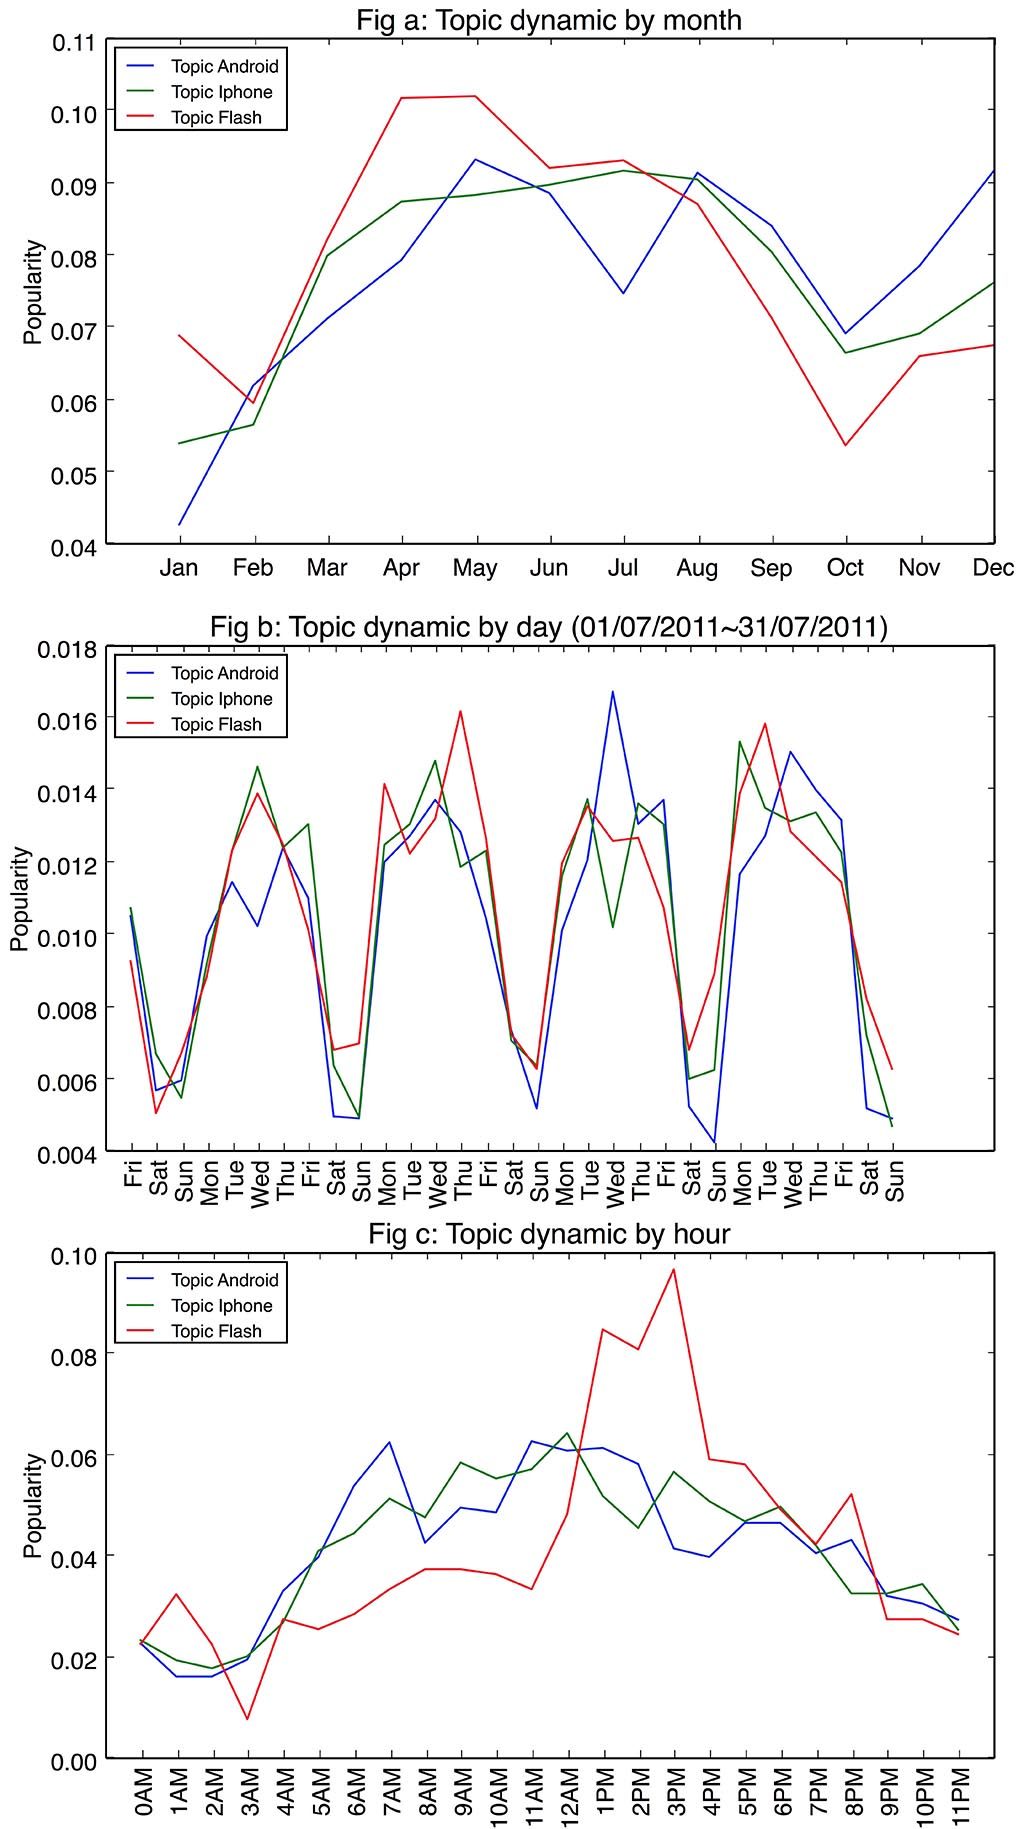
\includegraphics[width=5in]{timelevelv2.jpeg}  
\caption{Topic dynamics}
\label{fig:timelevel} 
\end{figure}
\begin{figure}
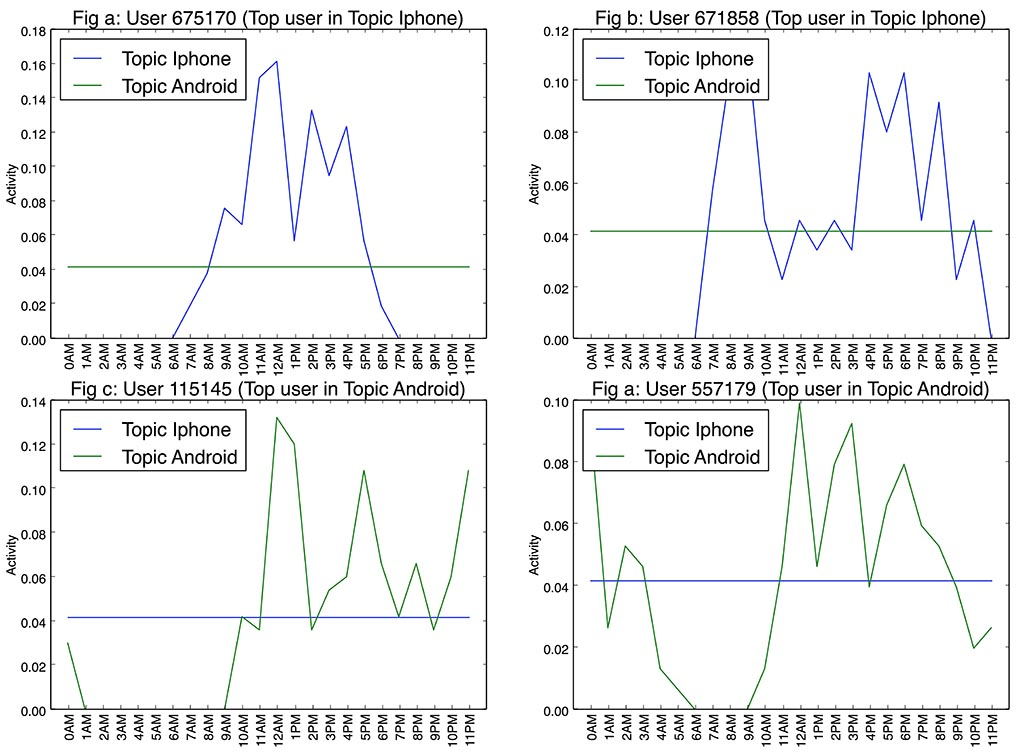
\includegraphics[width=5in]{timeusersmall.jpg}  
\caption{User Topic Activities}
\label{fig:usertimelevel} 
\end{figure}






\section{Summary: an effective model to extract expertise and temporal indications}
In this chapter, we addressed the problem of topic detection, activity modeling, temporal modeling and expertise detection in Q\&A sites. We presented the TTEA (Temporal Topic Expertise Activity) model that simultaneously uncovers the topics, activities, expertise and temporal dynamics. This extracted information can enable us to improve tasks such as: question routing, expert recommending and community life-cycle management. We demonstrated that TTEA shows advantages in topic modeling. It also achieves good performances on question routing task and expert detection task compared with the state of the art models. There are still many future directions for this work, for instances, it is obviously that the model is not limited to Q\&A datasets and we intend to adapt our model to other kinds of social media.
